\chapter{Treść pracy}
\label{sec:tresc}

\section{Użwanie pakietu \LaTeX}
\label{sec:tresc:latex}

	Informacje o tym jak używać pakietu \LaTeX można znaleźć w \cite{wiki:latex} i \cite{latex1}.\\

\section{Podział pracy na osobne pliki}
\label{sec:tresc:podzial}

Aby ułatwić pracę nad dokumentem, zwłaszcza w przypadku większej liczby zespołów warto go podzielić na większą ilość plików, na przykład według rozdziałów. W takim przypadku poszczególne rozdziały będą napisane w osobnych plikach tex, wstawianych do dokumentu głównego poleceniem $\backslash input$, na przykład:

%przykład wstawiania kodu:
\begin{lstlisting}
%\chapter{Wstęp}
\label{sec:wstep}
\textit{Autor: Mateusz Kowalski}

%===============================================================================
\section{Zawartość wstępu}
\label{sec:wstep:co}

\subsection{Opis zagadnienia poruszonego w pracy}
\sloppy
Pierwszy rozdział pracy powinien zawierać opis zagadnienia poruszonego w pracy.

\subsection{Rys historyczny i aktualne zastosowania}
\label{sec:wstep:rys}

Można również opisać historię badañ danego tematu, oraz jego aktualnych zastosowañ.

\subsection{Autorstwo pracy}
\textit{Autor: Rafał Kabaciñski}\\ \\
W przypadku pracy zespołowej pod tytułem każdego rozdziału powinno znaleźć się imię i nazwisko autora danego rozdziału. Autorem rozdziału może być tylko jedna osoba, ale podrozdziały mogą mieć innego autora niż cały rozdział. 

%===============================================================================
\section{Cel pracy}
\label{sec:wstep:cel}

	Wstęp powienien zawierać również rozdział opisujący cele projektu opisywanego w pracy jak na przykład:
	
\begin{itemize}
	\item zapoznanie się z informacjami na temat istniejących rozwiązañ,
	\item stworzenie funkcjonalnego urządzenia,
	\item sprawdzenie wybranych rozwiązañ konstrukcyjnych.
\end{itemize}

\section{Zawartość pracy}
\label{sec:wstep:zawartosc}
	
	Ostatecznie wstęp musi zawierać przewodnik opisujący co znajduje się w dalszych rozdziałach pracy. Na przykład:
	Ogólny zarys stanu wiedzy na temat przygotowania i składu prac dyplomowych przedstawiono w rozdziale drugim. W rozdziale trzecim wprowadzono podstawowe informacje na temat korzystania z tego formatu pracy. Rozdział czwarty stanowi podsumowanie pracy.

%\chapter{Stan wiedzy}
\label{sec:stanwiedzy}

Oprócz rozdziału opisującego rys historyczny (\ref{sec:wstep:rys}) konieczne jest również opisanie stanu wiedzy na temat danego zagadnienia. Powinno ono siê znaleźć w rozdziale drugim.

\section{Informacje dotyczące redakcji prac dyplomowych}
\label{sec:stanwiedzy:redakcja}

Informacje dotyczące zasad redakcji prac dyplomowych można znaleźć na stronie \url{www.cie.put.poznan.pl}.

%\chapter{Treść pracy}
\label{sec:tresc}

\section{Użwanie pakietu \LaTeX}
\label{sec:tresc:latex}

	Informacje o tym jak używać pakietu \LaTeX można znaleźć w \cite{wiki:latex} i \cite{latex1}.\\

\section{Podział pracy na osobne pliki}
\label{sec:tresc:podzial}

Aby ułatwić pracę nad dokumentem, zwłaszcza w przypadku większej liczby zespołów warto go podzielić na większą ilość plików, na przykład według rozdziałów. W takim przypadku poszczególne rozdziały będą napisane w osobnych plikach tex, wstawianych do dokumentu głównego poleceniem $\backslash input$, na przykład:

%przykład wstawiania kodu:
\begin{lstlisting}
%\chapter{Wstęp}
\label{sec:wstep}
\textit{Autor: Mateusz Kowalski}

%===============================================================================
\section{Zawartość wstępu}
\label{sec:wstep:co}

\subsection{Opis zagadnienia poruszonego w pracy}
\sloppy
Pierwszy rozdział pracy powinien zawierać opis zagadnienia poruszonego w pracy.

\subsection{Rys historyczny i aktualne zastosowania}
\label{sec:wstep:rys}

Można również opisać historię badañ danego tematu, oraz jego aktualnych zastosowañ.

\subsection{Autorstwo pracy}
\textit{Autor: Rafał Kabaciñski}\\ \\
W przypadku pracy zespołowej pod tytułem każdego rozdziału powinno znaleźć się imię i nazwisko autora danego rozdziału. Autorem rozdziału może być tylko jedna osoba, ale podrozdziały mogą mieć innego autora niż cały rozdział. 

%===============================================================================
\section{Cel pracy}
\label{sec:wstep:cel}

	Wstęp powienien zawierać również rozdział opisujący cele projektu opisywanego w pracy jak na przykład:
	
\begin{itemize}
	\item zapoznanie się z informacjami na temat istniejących rozwiązañ,
	\item stworzenie funkcjonalnego urządzenia,
	\item sprawdzenie wybranych rozwiązañ konstrukcyjnych.
\end{itemize}

\section{Zawartość pracy}
\label{sec:wstep:zawartosc}
	
	Ostatecznie wstęp musi zawierać przewodnik opisujący co znajduje się w dalszych rozdziałach pracy. Na przykład:
	Ogólny zarys stanu wiedzy na temat przygotowania i składu prac dyplomowych przedstawiono w rozdziale drugim. W rozdziale trzecim wprowadzono podstawowe informacje na temat korzystania z tego formatu pracy. Rozdział czwarty stanowi podsumowanie pracy.

%\chapter{Stan wiedzy}
\label{sec:stanwiedzy}

Oprócz rozdziału opisującego rys historyczny (\ref{sec:wstep:rys}) konieczne jest również opisanie stanu wiedzy na temat danego zagadnienia. Powinno ono siê znaleźć w rozdziale drugim.

\section{Informacje dotyczące redakcji prac dyplomowych}
\label{sec:stanwiedzy:redakcja}

Informacje dotyczące zasad redakcji prac dyplomowych można znaleźć na stronie \url{www.cie.put.poznan.pl}.

%\chapter{Treść pracy}
\label{sec:tresc}

\section{Użwanie pakietu \LaTeX}
\label{sec:tresc:latex}

	Informacje o tym jak używać pakietu \LaTeX można znaleźć w \cite{wiki:latex} i \cite{latex1}.\\

\section{Podział pracy na osobne pliki}
\label{sec:tresc:podzial}

Aby ułatwić pracę nad dokumentem, zwłaszcza w przypadku większej liczby zespołów warto go podzielić na większą ilość plików, na przykład według rozdziałów. W takim przypadku poszczególne rozdziały będą napisane w osobnych plikach tex, wstawianych do dokumentu głównego poleceniem $\backslash input$, na przykład:

%przykład wstawiania kodu:
\begin{lstlisting}
%\chapter{Wstęp}
\label{sec:wstep}
\textit{Autor: Mateusz Kowalski}

%===============================================================================
\section{Zawartość wstępu}
\label{sec:wstep:co}

\subsection{Opis zagadnienia poruszonego w pracy}
\sloppy
Pierwszy rozdział pracy powinien zawierać opis zagadnienia poruszonego w pracy.

\subsection{Rys historyczny i aktualne zastosowania}
\label{sec:wstep:rys}

Można również opisać historię badañ danego tematu, oraz jego aktualnych zastosowañ.

\subsection{Autorstwo pracy}
\textit{Autor: Rafał Kabaciñski}\\ \\
W przypadku pracy zespołowej pod tytułem każdego rozdziału powinno znaleźć się imię i nazwisko autora danego rozdziału. Autorem rozdziału może być tylko jedna osoba, ale podrozdziały mogą mieć innego autora niż cały rozdział. 

%===============================================================================
\section{Cel pracy}
\label{sec:wstep:cel}

	Wstęp powienien zawierać również rozdział opisujący cele projektu opisywanego w pracy jak na przykład:
	
\begin{itemize}
	\item zapoznanie się z informacjami na temat istniejących rozwiązañ,
	\item stworzenie funkcjonalnego urządzenia,
	\item sprawdzenie wybranych rozwiązañ konstrukcyjnych.
\end{itemize}

\section{Zawartość pracy}
\label{sec:wstep:zawartosc}
	
	Ostatecznie wstęp musi zawierać przewodnik opisujący co znajduje się w dalszych rozdziałach pracy. Na przykład:
	Ogólny zarys stanu wiedzy na temat przygotowania i składu prac dyplomowych przedstawiono w rozdziale drugim. W rozdziale trzecim wprowadzono podstawowe informacje na temat korzystania z tego formatu pracy. Rozdział czwarty stanowi podsumowanie pracy.

%\chapter{Stan wiedzy}
\label{sec:stanwiedzy}

Oprócz rozdziału opisującego rys historyczny (\ref{sec:wstep:rys}) konieczne jest również opisanie stanu wiedzy na temat danego zagadnienia. Powinno ono siê znaleźć w rozdziale drugim.

\section{Informacje dotyczące redakcji prac dyplomowych}
\label{sec:stanwiedzy:redakcja}

Informacje dotyczące zasad redakcji prac dyplomowych można znaleźć na stronie \url{www.cie.put.poznan.pl}.

%\chapter{Treść pracy}
\label{sec:tresc}

\section{Użwanie pakietu \LaTeX}
\label{sec:tresc:latex}

	Informacje o tym jak używać pakietu \LaTeX można znaleźć w \cite{wiki:latex} i \cite{latex1}.\\

\section{Podział pracy na osobne pliki}
\label{sec:tresc:podzial}

Aby ułatwić pracę nad dokumentem, zwłaszcza w przypadku większej liczby zespołów warto go podzielić na większą ilość plików, na przykład według rozdziałów. W takim przypadku poszczególne rozdziały będą napisane w osobnych plikach tex, wstawianych do dokumentu głównego poleceniem $\backslash input$, na przykład:

%przykład wstawiania kodu:
\begin{lstlisting}
%\input{01-Wstep.tex}
%\input{02-Stanwiedzy.tex}
%\input{03-Tresc.tex}
%\input{04-Wnioski.tex}
\end{lstlisting}

\section{Wzory matematyczne w \LaTeX}
\label{sec:tresc:wzory}

Przykładowy wzór: odwrotna transformata Fouriera:

\begin{itemize}
\item Ciągła:

\begin{equation}
 f(x) = \mathcal{F}^{-1}\{\hat{f}(\xi)\} = \int\limits_{-\infty}^{\infty}\hat{f}(\xi)e^{2\pi ix\xi}dx
 \label{eq:f2}
\end{equation}

\item Dyskretna:

\begin{equation}
 f(n) = \frac{1}{N}\sum\limits_{k = 0}^{N-1}F_{DFT}(k)e^{j \frac{2\pi}{N}nk}dx
 \label{eq:f4}
\end{equation}

\end{itemize}

Przykładowa macierz: elementarna macierz obrotu punktu wokół osi $x$ o kąt $\alpha$:

$$RotX(\alpha) = \left[ \begin{array}{c c c} 
1 & 0 & 0 \\
0 & cos(\alpha) & -sin(\alpha) \\ 
0 & sin(\alpha) & cos(\alpha)
\end{array} \right] $$

\section{Tabele}
\label{sec:tresc:tab}

Tabela \ref{tab1} zawiera przykładowe wyniki dwóch sprawdzianów.

\begin{table}[h]
	\begin{center}
	\caption{Przykladowa tabela}
	\label{tab1}
	\begin{tabular}{|c|c|c|c|}
		\hline
		Lp.& nr indeksu & \multicolumn{2}{|c|}{kolokwium}\\ \cline{3-4}
		   &            & I   & II \\ \hline
		1  & 32453      & 4,0  & 5,0\\
		2  & 42546      & 3,5  & 4,0\\
		3  & 32546      & 2,0  & 3,0\\ \hline
	\end{tabular}
	\end{center}
\end{table}

\section{Rysunki}
\label{sec:tresc:rys}

Rysunek \ref{fig:rys1} zawiera logo Politechniki Poznañskiej.\\

\begin{figure}[h]
	\begin{center}
		
\includegraphics[height = 3cm]{figures/template/logo-pp}
		\caption[Logo Politechniki Poznañskiej]{Logo Politechniki Poznañskiej; uwaga: w podpisach rysunków nie ma kropek na koñcu zdania; jeżeli zdañ jest więcej należy oddzielać je średnikami i zaczynać z małej litery}

		\label{fig:rys1}
	\end{center}
\end{figure}

\section{Dodawanie pakietów}
\label{sec:tresc:pakiety}

W przypadku użycia pakietu MiKTeX, aby zainstalować dodatkowe pakiety należy włączyć {\itshape Package Manager}, w katalogu {\itshape Maintenance (Admin)}. Następnie w pole {\itshape Name} wpisać nazwę brakującego pakietu i nacisnąć przycisk {\itshape Filter}. Nazwę wybranego pakietu należy kliknąć prawym przyciskiem myszy i nacisnąć {\itshape Install}, jak na rysunku \ref{fig:pakiety}.

\begin{figure}[h]
	\begin{center}
		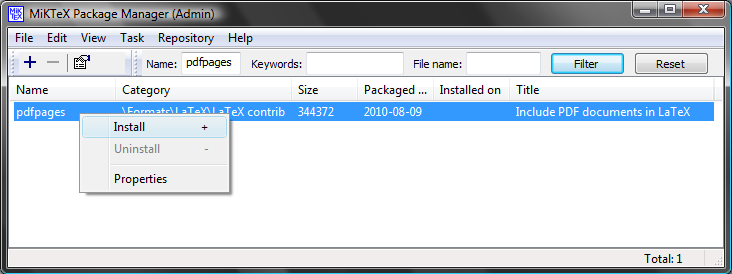
\includegraphics[width = 12cm]{figures/pakiety.png}
		\caption{Instalacja dodatkowych pakietów}
		\label{fig:pakiety}
	\end{center}
\end{figure}

\section{Pakiet Bib\TeX}
\label{sec:tresc:bibtex}

Pakiet Bib\TeX służy do zarządzania bibliografią. Pozycje bibliograficzne zapisywane są w plikach tekstowych z rozszerzeniem $.bib$, a następnie wywołanie poleceniem $\backslash cite$. Pliki bib muszą mieć odpowiednią strukturę, którą można poznać na stronie \url{http://pl.wikipedia.org/wiki/BibTeX}, lub \url{http://en.wikipedia.org/wiki/BibTeX}.\\
Bibliografię tworzy się wywołując w dokumencie polecenie $\backslash bibliography$. Po skompilowaniu dokumentu zawierającego odwołania do bibliografii, należy skompilować bibliografię za pomocą osobnego przycisku, a następnie znów skompilować dokument. Kompiluje się jednak zawsze tylko z widoku głównego dokumentu. Bib\TeX sam uporządkuje bibliografię według podanego stylu, zamieszczając tylko te pozycje które zostały zacytowane. Styl bibliografii ustawiany jest poleceniem $\backslash bibliographystyle$ przed wywołaniem pierwszego cytowania. W tym dokumencie użyto stylu plplain.

%
\chapter{Podsumowanie}
\label{sec:podsumowanie}

W podsumowaniu należy pokrótce opisać sposoby i efekty realizacji celów pracy przedstawionych w rozdziale \ref{sec:wstep:cel}. Oprócz tego powinny siê tu znaleść wnioski wynikające z wyników pracy, oraz dalsze kierunki rozwoju zagadnienia.

\end{lstlisting}

\section{Wzory matematyczne w \LaTeX}
\label{sec:tresc:wzory}

Przykładowy wzór: odwrotna transformata Fouriera:

\begin{itemize}
\item Ciągła:

\begin{equation}
 f(x) = \mathcal{F}^{-1}\{\hat{f}(\xi)\} = \int\limits_{-\infty}^{\infty}\hat{f}(\xi)e^{2\pi ix\xi}dx
 \label{eq:f2}
\end{equation}

\item Dyskretna:

\begin{equation}
 f(n) = \frac{1}{N}\sum\limits_{k = 0}^{N-1}F_{DFT}(k)e^{j \frac{2\pi}{N}nk}dx
 \label{eq:f4}
\end{equation}

\end{itemize}

Przykładowa macierz: elementarna macierz obrotu punktu wokół osi $x$ o kąt $\alpha$:

$$RotX(\alpha) = \left[ \begin{array}{c c c} 
1 & 0 & 0 \\
0 & cos(\alpha) & -sin(\alpha) \\ 
0 & sin(\alpha) & cos(\alpha)
\end{array} \right] $$

\section{Tabele}
\label{sec:tresc:tab}

Tabela \ref{tab1} zawiera przykładowe wyniki dwóch sprawdzianów.

\begin{table}[h]
	\begin{center}
	\caption{Przykladowa tabela}
	\label{tab1}
	\begin{tabular}{|c|c|c|c|}
		\hline
		Lp.& nr indeksu & \multicolumn{2}{|c|}{kolokwium}\\ \cline{3-4}
		   &            & I   & II \\ \hline
		1  & 32453      & 4,0  & 5,0\\
		2  & 42546      & 3,5  & 4,0\\
		3  & 32546      & 2,0  & 3,0\\ \hline
	\end{tabular}
	\end{center}
\end{table}

\section{Rysunki}
\label{sec:tresc:rys}

Rysunek \ref{fig:rys1} zawiera logo Politechniki Poznañskiej.\\

\begin{figure}[h]
	\begin{center}
		
\includegraphics[height = 3cm]{figures/template/logo-pp}
		\caption[Logo Politechniki Poznañskiej]{Logo Politechniki Poznañskiej; uwaga: w podpisach rysunków nie ma kropek na koñcu zdania; jeżeli zdañ jest więcej należy oddzielać je średnikami i zaczynać z małej litery}

		\label{fig:rys1}
	\end{center}
\end{figure}

\section{Dodawanie pakietów}
\label{sec:tresc:pakiety}

W przypadku użycia pakietu MiKTeX, aby zainstalować dodatkowe pakiety należy włączyć {\itshape Package Manager}, w katalogu {\itshape Maintenance (Admin)}. Następnie w pole {\itshape Name} wpisać nazwę brakującego pakietu i nacisnąć przycisk {\itshape Filter}. Nazwę wybranego pakietu należy kliknąć prawym przyciskiem myszy i nacisnąć {\itshape Install}, jak na rysunku \ref{fig:pakiety}.

\begin{figure}[h]
	\begin{center}
		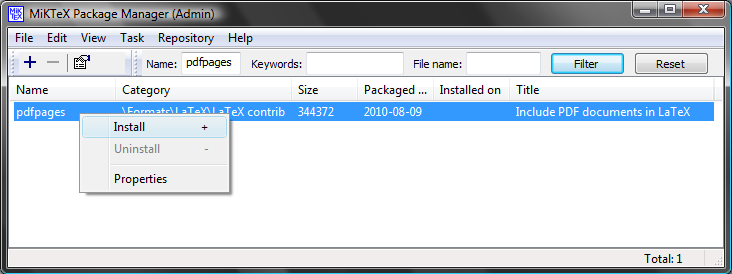
\includegraphics[width = 12cm]{figures/pakiety.png}
		\caption{Instalacja dodatkowych pakietów}
		\label{fig:pakiety}
	\end{center}
\end{figure}

\section{Pakiet Bib\TeX}
\label{sec:tresc:bibtex}

Pakiet Bib\TeX służy do zarządzania bibliografią. Pozycje bibliograficzne zapisywane są w plikach tekstowych z rozszerzeniem $.bib$, a następnie wywołanie poleceniem $\backslash cite$. Pliki bib muszą mieć odpowiednią strukturę, którą można poznać na stronie \url{http://pl.wikipedia.org/wiki/BibTeX}, lub \url{http://en.wikipedia.org/wiki/BibTeX}.\\
Bibliografię tworzy się wywołując w dokumencie polecenie $\backslash bibliography$. Po skompilowaniu dokumentu zawierającego odwołania do bibliografii, należy skompilować bibliografię za pomocą osobnego przycisku, a następnie znów skompilować dokument. Kompiluje się jednak zawsze tylko z widoku głównego dokumentu. Bib\TeX sam uporządkuje bibliografię według podanego stylu, zamieszczając tylko te pozycje które zostały zacytowane. Styl bibliografii ustawiany jest poleceniem $\backslash bibliographystyle$ przed wywołaniem pierwszego cytowania. W tym dokumencie użyto stylu plplain.

%
\chapter{Podsumowanie}
\label{sec:podsumowanie}

W podsumowaniu należy pokrótce opisać sposoby i efekty realizacji celów pracy przedstawionych w rozdziale \ref{sec:wstep:cel}. Oprócz tego powinny siê tu znaleść wnioski wynikające z wyników pracy, oraz dalsze kierunki rozwoju zagadnienia.

\end{lstlisting}

\section{Wzory matematyczne w \LaTeX}
\label{sec:tresc:wzory}

Przykładowy wzór: odwrotna transformata Fouriera:

\begin{itemize}
\item Ciągła:

\begin{equation}
 f(x) = \mathcal{F}^{-1}\{\hat{f}(\xi)\} = \int\limits_{-\infty}^{\infty}\hat{f}(\xi)e^{2\pi ix\xi}dx
 \label{eq:f2}
\end{equation}

\item Dyskretna:

\begin{equation}
 f(n) = \frac{1}{N}\sum\limits_{k = 0}^{N-1}F_{DFT}(k)e^{j \frac{2\pi}{N}nk}dx
 \label{eq:f4}
\end{equation}

\end{itemize}

Przykładowa macierz: elementarna macierz obrotu punktu wokół osi $x$ o kąt $\alpha$:

$$RotX(\alpha) = \left[ \begin{array}{c c c} 
1 & 0 & 0 \\
0 & cos(\alpha) & -sin(\alpha) \\ 
0 & sin(\alpha) & cos(\alpha)
\end{array} \right] $$

\section{Tabele}
\label{sec:tresc:tab}

Tabela \ref{tab1} zawiera przykładowe wyniki dwóch sprawdzianów.

\begin{table}[h]
	\begin{center}
	\caption{Przykladowa tabela}
	\label{tab1}
	\begin{tabular}{|c|c|c|c|}
		\hline
		Lp.& nr indeksu & \multicolumn{2}{|c|}{kolokwium}\\ \cline{3-4}
		   &            & I   & II \\ \hline
		1  & 32453      & 4,0  & 5,0\\
		2  & 42546      & 3,5  & 4,0\\
		3  & 32546      & 2,0  & 3,0\\ \hline
	\end{tabular}
	\end{center}
\end{table}

\section{Rysunki}
\label{sec:tresc:rys}

Rysunek \ref{fig:rys1} zawiera logo Politechniki Poznañskiej.\\

\begin{figure}[h]
	\begin{center}
		
\includegraphics[height = 3cm]{figures/template/logo-pp}
		\caption[Logo Politechniki Poznañskiej]{Logo Politechniki Poznañskiej; uwaga: w podpisach rysunków nie ma kropek na koñcu zdania; jeżeli zdañ jest więcej należy oddzielać je średnikami i zaczynać z małej litery}

		\label{fig:rys1}
	\end{center}
\end{figure}

\section{Dodawanie pakietów}
\label{sec:tresc:pakiety}

W przypadku użycia pakietu MiKTeX, aby zainstalować dodatkowe pakiety należy włączyć {\itshape Package Manager}, w katalogu {\itshape Maintenance (Admin)}. Następnie w pole {\itshape Name} wpisać nazwę brakującego pakietu i nacisnąć przycisk {\itshape Filter}. Nazwę wybranego pakietu należy kliknąć prawym przyciskiem myszy i nacisnąć {\itshape Install}, jak na rysunku \ref{fig:pakiety}.

\begin{figure}[h]
	\begin{center}
		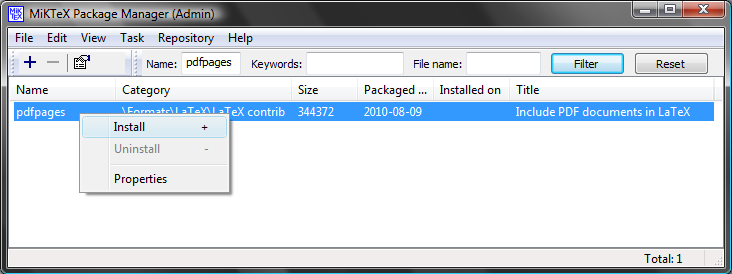
\includegraphics[width = 12cm]{figures/pakiety.png}
		\caption{Instalacja dodatkowych pakietów}
		\label{fig:pakiety}
	\end{center}
\end{figure}

\section{Pakiet Bib\TeX}
\label{sec:tresc:bibtex}

Pakiet Bib\TeX służy do zarządzania bibliografią. Pozycje bibliograficzne zapisywane są w plikach tekstowych z rozszerzeniem $.bib$, a następnie wywołanie poleceniem $\backslash cite$. Pliki bib muszą mieć odpowiednią strukturę, którą można poznać na stronie \url{http://pl.wikipedia.org/wiki/BibTeX}, lub \url{http://en.wikipedia.org/wiki/BibTeX}.\\
Bibliografię tworzy się wywołując w dokumencie polecenie $\backslash bibliography$. Po skompilowaniu dokumentu zawierającego odwołania do bibliografii, należy skompilować bibliografię za pomocą osobnego przycisku, a następnie znów skompilować dokument. Kompiluje się jednak zawsze tylko z widoku głównego dokumentu. Bib\TeX sam uporządkuje bibliografię według podanego stylu, zamieszczając tylko te pozycje które zostały zacytowane. Styl bibliografii ustawiany jest poleceniem $\backslash bibliographystyle$ przed wywołaniem pierwszego cytowania. W tym dokumencie użyto stylu plplain.

%
\chapter{Podsumowanie}
\label{sec:podsumowanie}

W podsumowaniu należy pokrótce opisać sposoby i efekty realizacji celów pracy przedstawionych w rozdziale \ref{sec:wstep:cel}. Oprócz tego powinny siê tu znaleść wnioski wynikające z wyników pracy, oraz dalsze kierunki rozwoju zagadnienia.

\end{lstlisting}

\section{Wzory matematyczne w \LaTeX}
\label{sec:tresc:wzory}

Przykładowy wzór: odwrotna transformata Fouriera:

\begin{itemize}
\item Ciągła:

\begin{equation}
 f(x) = \mathcal{F}^{-1}\{\hat{f}(\xi)\} = \int\limits_{-\infty}^{\infty}\hat{f}(\xi)e^{2\pi ix\xi}dx
 \label{eq:f2}
\end{equation}

\item Dyskretna:

\begin{equation}
 f(n) = \frac{1}{N}\sum\limits_{k = 0}^{N-1}F_{DFT}(k)e^{j \frac{2\pi}{N}nk}dx
 \label{eq:f4}
\end{equation}

\end{itemize}

Przykładowa macierz: elementarna macierz obrotu punktu wokół osi $x$ o kąt $\alpha$:

$$RotX(\alpha) = \left[ \begin{array}{c c c} 
1 & 0 & 0 \\
0 & cos(\alpha) & -sin(\alpha) \\ 
0 & sin(\alpha) & cos(\alpha)
\end{array} \right] $$

\section{Tabele}
\label{sec:tresc:tab}

Tabela \ref{tab1} zawiera przykładowe wyniki dwóch sprawdzianów.

\begin{table}[h]
	\begin{center}
	\caption{Przykladowa tabela}
	\label{tab1}
	\begin{tabular}{|c|c|c|c|}
		\hline
		Lp.& nr indeksu & \multicolumn{2}{|c|}{kolokwium}\\ \cline{3-4}
		   &            & I   & II \\ \hline
		1  & 32453      & 4,0  & 5,0\\
		2  & 42546      & 3,5  & 4,0\\
		3  & 32546      & 2,0  & 3,0\\ \hline
	\end{tabular}
	\end{center}
\end{table}

\section{Rysunki}
\label{sec:tresc:rys}

Rysunek \ref{fig:rys1} zawiera logo Politechniki Poznañskiej.\\

\begin{figure}[h]
	\begin{center}
		
\includegraphics[height = 3cm]{figures/template/logo-pp}
		\caption[Logo Politechniki Poznañskiej]{Logo Politechniki Poznañskiej; uwaga: w podpisach rysunków nie ma kropek na koñcu zdania; jeżeli zdañ jest więcej należy oddzielać je średnikami i zaczynać z małej litery}

		\label{fig:rys1}
	\end{center}
\end{figure}

\section{Dodawanie pakietów}
\label{sec:tresc:pakiety}

W przypadku użycia pakietu MiKTeX, aby zainstalować dodatkowe pakiety należy włączyć {\itshape Package Manager}, w katalogu {\itshape Maintenance (Admin)}. Następnie w pole {\itshape Name} wpisać nazwę brakującego pakietu i nacisnąć przycisk {\itshape Filter}. Nazwę wybranego pakietu należy kliknąć prawym przyciskiem myszy i nacisnąć {\itshape Install}, jak na rysunku \ref{fig:pakiety}.

\begin{figure}[h]
	\begin{center}
		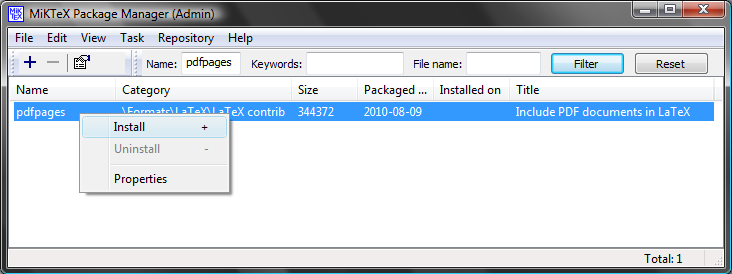
\includegraphics[width = 12cm]{figures/pakiety.png}
		\caption{Instalacja dodatkowych pakietów}
		\label{fig:pakiety}
	\end{center}
\end{figure}

\section{Pakiet Bib\TeX}
\label{sec:tresc:bibtex}

Pakiet Bib\TeX służy do zarządzania bibliografią. Pozycje bibliograficzne zapisywane są w plikach tekstowych z rozszerzeniem $.bib$, a następnie wywołanie poleceniem $\backslash cite$. Pliki bib muszą mieć odpowiednią strukturę, którą można poznać na stronie \url{http://pl.wikipedia.org/wiki/BibTeX}, lub \url{http://en.wikipedia.org/wiki/BibTeX}.\\
Bibliografię tworzy się wywołując w dokumencie polecenie $\backslash bibliography$. Po skompilowaniu dokumentu zawierającego odwołania do bibliografii, należy skompilować bibliografię za pomocą osobnego przycisku, a następnie znów skompilować dokument. Kompiluje się jednak zawsze tylko z widoku głównego dokumentu. Bib\TeX sam uporządkuje bibliografię według podanego stylu, zamieszczając tylko te pozycje które zostały zacytowane. Styl bibliografii ustawiany jest poleceniem $\backslash bibliographystyle$ przed wywołaniem pierwszego cytowania. W tym dokumencie użyto stylu plplain.
